\section{Introduction}
\label{sec:intro}

\IEEEPARstart{N}{avigating} dynamic, human-populated environments is a fundamental challenge in embodied AI and mobile robotics. A truly autonomous home or service robot must not only avoid physical collisions but also adhere to implicit social norms. This includes maintaining a polite distance from a conversation, yielding to a person approaching from a blind corner, or proactively responding to an acoustic target such as a doorbell ringing or a human calling for help. While humans naturally rely on a rich, synchronized fusion of visual and acoustic cues to navigate these complex social dynamics, current robotic navigation systems often process these modalities in isolation, severely limiting their social intelligence.

\begin{figure}[t]
    \centering
    % TODO: Replace with the actual teaser figure once updated
    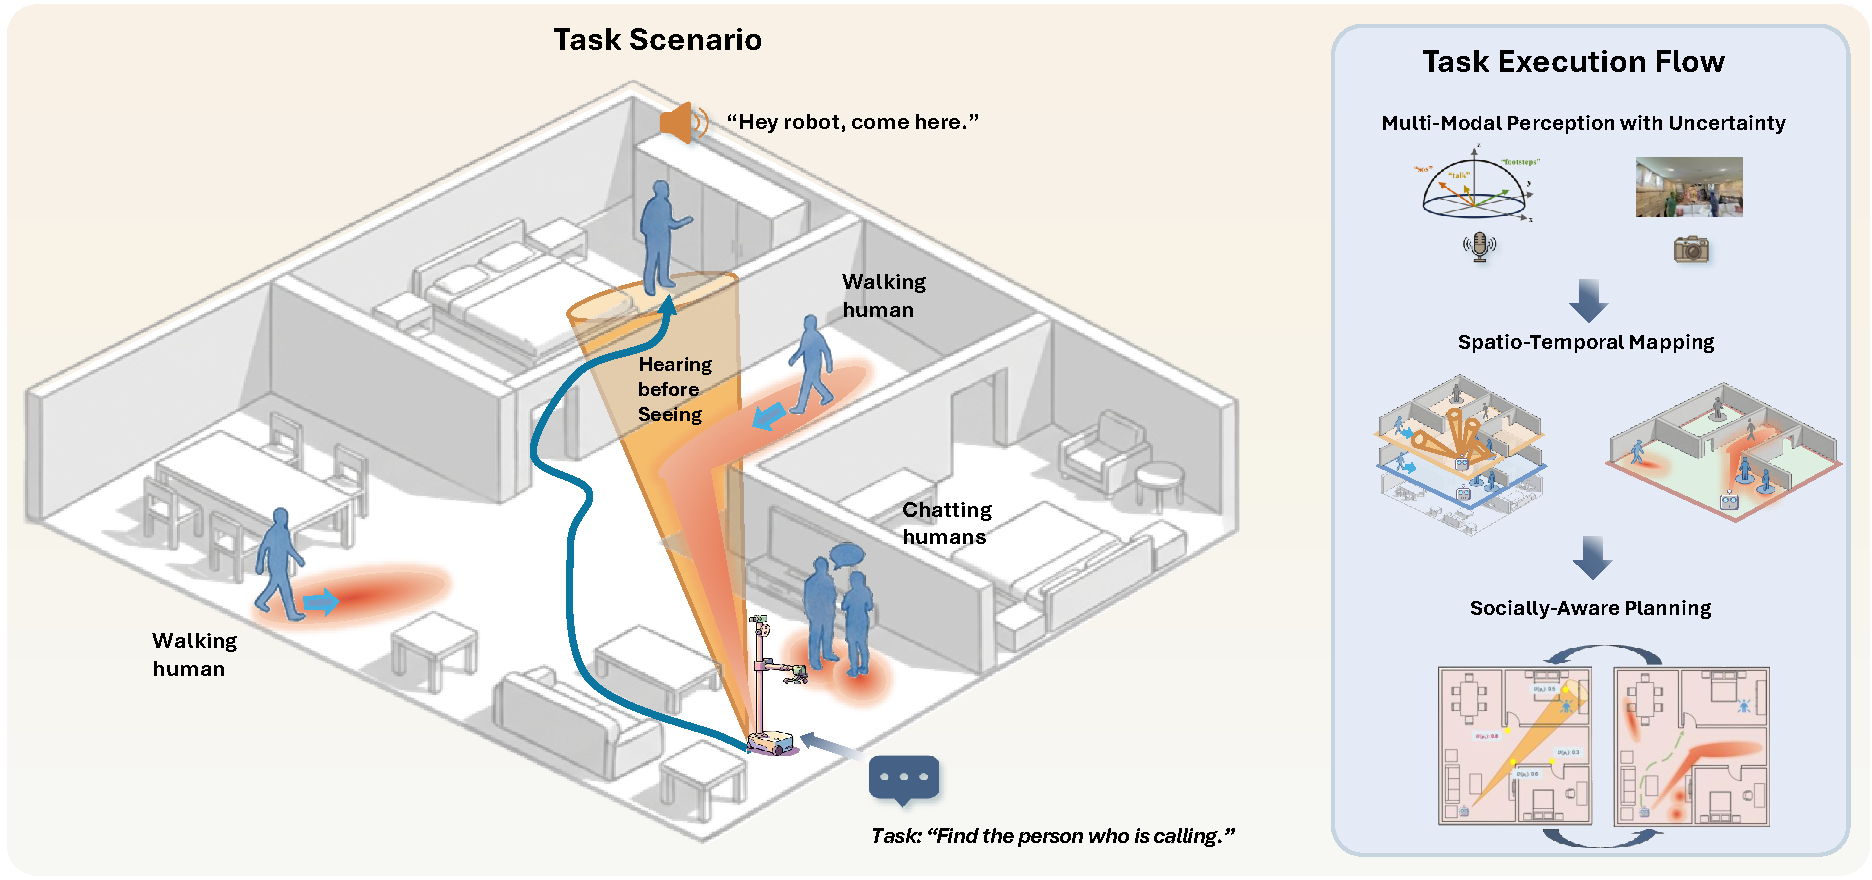
\includegraphics[width=0.99\linewidth]{figures/teaser.pdf}
    \caption{Overview of SAVNav, our socially-aware audio-visual navigation framework. Traditional visual social navigation (red dashed line) is ``deaf'' to occluded events, and socially-unaware AVNav simply treats sound as a geometric target. In contrast, SAVNav (blue solid line) ``hears'' the environment's social context. By localizing conversations and footsteps (colored acoustic cones), the robot models them as dynamic social boundaries to proactively yield, while simultaneously pursuing the acoustic target (e.g., a call for help).}
    \label{fig:teaser}
\end{figure}

Existing approaches to human-aware navigation broadly fall into two decoupled paradigms. On one hand, social navigation (SocialNav) predominantly relies on line-of-sight visual sensors (RGB-D, LiDAR) to detect pedestrians and forecast their trajectories. However, these systems are fundamentally ``deaf''; they cannot anticipate a person walking behind a wall via footstep sounds or recognize a stationary group engaged in conversation, often leading to intrusive, startling, or unsafe behaviors. On the other hand, audio-visual navigation (AVNav) leverages binaural or multi-channel audio to locate sound sources (e.g., AudioGoal). Yet, these methods typically treat audio purely as a geometric target to reach or as background noise to ignore. They lack the social awareness required to treat social acoustic events as dynamic social boundaries.

To bridge the gap between deaf social navigation and socially-unaware AVNav, we introduce SAVNav, a novel framework for socially-aware audio-visual navigation. As illustrated in Fig.~\ref{fig:teaser}, SAVNav is a comprehensive sensorimotor framework that elevates social acoustic events from physical signals to semantic social constraints. Recognizing that our task requires innovations across perception, mapping, and planning, we architect SAVNav as a tightly integrated pipeline.

In the perception module, we integrate first-order Ambisonics (FOA) acoustic positioning (via Embed-ACCDOA~\cite{OpenvocabularySoundEvent2025}) with RGB-D visual abstraction (YOLO26 and ImageBind) to extract both the spatial location and semantic category of sound events and human activities. These multi-modal streams are then dynamically fused into SAVMap, a novel spatio-temporal representation that features a robust sparse audio-visual anchoring mechanism for multi-modal alignment and a topology-aware acoustic anticipation algorithm. This allows the system to anticipate non-line-of-sight (NLOS) dynamic pedestrians (DPs) from social acoustic events, mapping them into dynamic, anisotropic social cost fields. Finally, our planning layer employs the SAVNav policy. Rather than passively following geometric shortest paths, the robot proactively explores the environment to resolve acoustic ambiguities of the acoustic target, while simultaneously anticipating and yielding to the dynamic social boundaries defined by human activities.

The main contributions of this work are summarized as follows:
\begin{enumerate}
    \item \textit{A Novel Benchmark for the SAVNav Task:} We introduce a new task where embodied agents must locate an acoustic target while simultaneously interpreting social acoustic events (e.g., conversations, footsteps) as dynamic social boundaries. To support this, we develop a high-fidelity continuous simulation environment with multi-agent human dynamics and complex acoustic rendering, accompanied by a comprehensive dataset and new social compliance metrics.
    \item \textit{Acoustic-to-Spatial Social Mapping (SAVMap):} We propose SAVMap, a spatio-temporal representation that transforms human-generated sounds, including non-line-of-sight (NLOS) acoustic events, into persistent spatial social constraints. By fusing audio observations with visual cues and scene topology, SAVMap enables the robot to infer NLOS social boundaries and dynamic pedestrians (DPs) before visual confirmation.
    \item \textit{Proactive Socially-Aware Navigation Policy (SAVNav Policy):} We design the SAVNav policy, a planning module that uses SAVMap to proactively yield to inferred social boundaries while actively disambiguating uncertain observations of the acoustic target when necessary, enabling robust target reaching in dynamic human environments.
    \item \textit{Extensive Evaluation:} Extensive evaluations in our simulated benchmark and deployments on a physical Stretch 3 robot demonstrate that SAVNav significantly outperforms state-of-the-art visual-only and audio-visual baselines in navigation success, search efficiency, and social compliance.
\end{enumerate}
